\documentclass[1p]{elsarticle_modified}
%\bibliographystyle{elsarticle-num}

%\usepackage[colorlinks]{hyperref}
%\usepackage{abbrmath_seonhwa} %\Abb, \Ascr, \Acal ,\Abf, \Afrak
\usepackage{amsfonts}
\usepackage{amssymb}
\usepackage{amsmath}
\usepackage{amsthm}
\usepackage{scalefnt}
\usepackage{amsbsy}
\usepackage{kotex}
\usepackage{caption}
\usepackage{subfig}
\usepackage{color}
\usepackage{graphicx}
\usepackage{xcolor} %% white, black, red, green, blue, cyan, magenta, yellow
\usepackage{float}
\usepackage{setspace}
\usepackage{hyperref}

\usepackage{tikz}
\usetikzlibrary{arrows}

\usepackage{multirow}
\usepackage{array} % fixed length table
\usepackage{hhline}

%%%%%%%%%%%%%%%%%%%%%
\makeatletter
\renewcommand*\env@matrix[1][\arraystretch]{%
	\edef\arraystretch{#1}%
	\hskip -\arraycolsep
	\let\@ifnextchar\new@ifnextchar
	\array{*\c@MaxMatrixCols c}}
\makeatother %https://tex.stackexchange.com/questions/14071/how-can-i-increase-the-line-spacing-in-a-matrix
%%%%%%%%%%%%%%%

\usepackage[normalem]{ulem}

\newcommand{\msout}[1]{\ifmmode\text{\sout{\ensuremath{#1}}}\else\sout{#1}\fi}
%SOURCE: \msout is \stkout macro in https://tex.stackexchange.com/questions/20609/strikeout-in-math-mode

\newcommand{\cancel}[1]{
	\ifmmode
	{\color{red}\msout{#1}}
	\else
	{\color{red}\sout{#1}}
	\fi
}

\newcommand{\add}[1]{
	{\color{blue}\uwave{#1}}
}

\newcommand{\replace}[2]{
	\ifmmode
	{\color{red}\msout{#1}}{\color{blue}\uwave{#2}}
	\else
	{\color{red}\sout{#1}}{\color{blue}\uwave{#2}}
	\fi
}

\newcommand{\Sol}{\mathcal{S}} %segment
\newcommand{\D}{D} %diagram
\newcommand{\A}{\mathcal{A}} %arc


%%%%%%%%%%%%%%%%%%%%%%%%%%%%%5 test

\def\sl{\operatorname{\textup{SL}}(2,\Cbb)}
\def\psl{\operatorname{\textup{PSL}}(2,\Cbb)}
\def\quan{\mkern 1mu \triangleright \mkern 1mu}

\theoremstyle{definition}
\newtheorem{thm}{Theorem}[section]
\newtheorem{prop}[thm]{Proposition}
\newtheorem{lem}[thm]{Lemma}
\newtheorem{ques}[thm]{Question}
\newtheorem{cor}[thm]{Corollary}
\newtheorem{defn}[thm]{Definition}
\newtheorem{exam}[thm]{Example}
\newtheorem{rmk}[thm]{Remark}
\newtheorem{alg}[thm]{Algorithm}

\newcommand{\I}{\sqrt{-1}}
\begin{document}

%\begin{frontmatter}
%
%\title{Boundary parabolic representations of knots up to 8 crossings}
%
%%% Group authors per affiliation:
%\author{Yunhi Cho} 
%\address{Department of Mathematics, University of Seoul, Seoul, Korea}
%\ead{yhcho@uos.ac.kr}
%
%
%\author{Seonhwa Kim} %\fnref{s_kim}}
%\address{Center for Geometry and Physics, Institute for Basic Science, Pohang, 37673, Korea}
%\ead{ryeona17@ibs.re.kr}
%
%\author{Hyuk Kim}
%\address{Department of Mathematical Sciences, Seoul National University, Seoul 08826, Korea}
%\ead{hyukkim@snu.ac.kr}
%
%\author{Seokbeom Yoon}
%\address{Department of Mathematical Sciences, Seoul National University, Seoul, 08826,  Korea}
%\ead{sbyoon15@snu.ac.kr}
%
%\begin{abstract}
%We find all boundary parabolic representation of knots up to 8 crossings.
%
%\end{abstract}
%\begin{keyword}
%    \MSC[2010] 57M25 
%\end{keyword}
%
%\end{frontmatter}

%\linenumbers
%\tableofcontents
%
\newcommand\colored[1]{\textcolor{white}{\rule[-0.35ex]{0.8em}{1.4ex}}\kern-0.8em\color{red} #1}%
%\newcommand\colored[1]{\textcolor{white}{ #1}\kern-2.17ex	\textcolor{white}{ #1}\kern-1.81ex	\textcolor{white}{ #1}\kern-2.15ex\color{red}#1	}

{\Large $\underline{12a_{0055}~(K12a_{0055})}$}

\setlength{\tabcolsep}{10pt}
\renewcommand{\arraystretch}{1.6}
\vspace{1cm}\begin{tabular}{m{100pt}>{\centering\arraybackslash}m{274pt}}
\multirow{5}{120pt}{
	\centering
	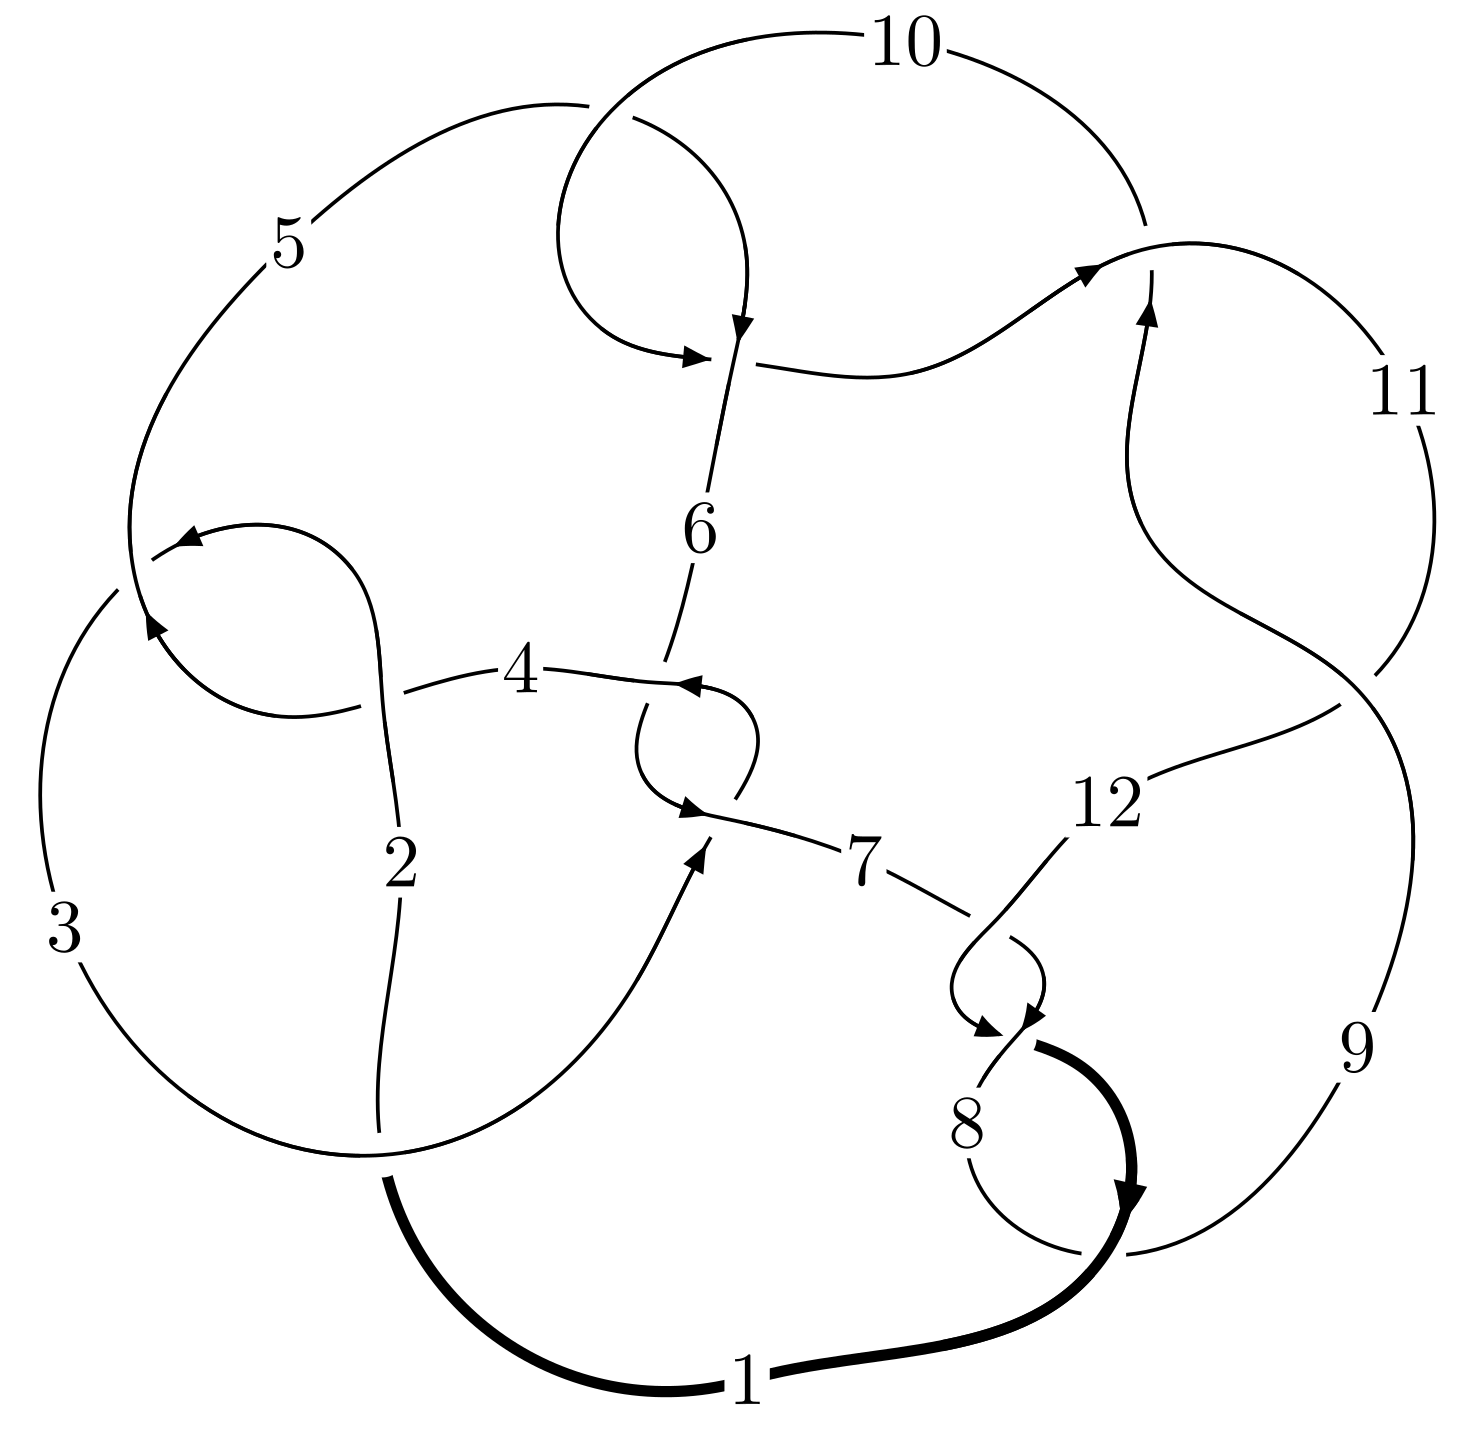
\includegraphics[width=112pt]{../../../GIT/diagram.site/Diagrams/png/856_12a_0055.png}\\
\ \ \ A knot diagram\footnotemark}&
\allowdisplaybreaks
\textbf{Linearized knot diagam} \\
\cline{2-2}
 &
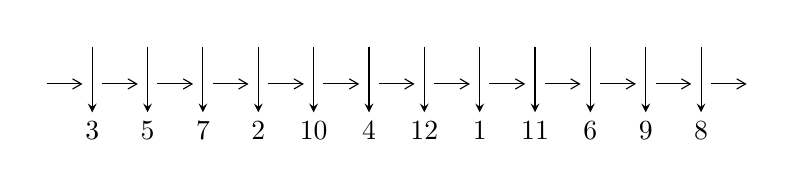
\begin{tikzpicture}[x=20pt, y=17pt]
	% nodes
	\node (C0) at (0, 0) {};
	\node (C1) at (1, 0) {};
	\node (C1U) at (1, +1) {};
	\node (C1D) at (1, -1) {3};

	\node (C2) at (2, 0) {};
	\node (C2U) at (2, +1) {};
	\node (C2D) at (2, -1) {5};

	\node (C3) at (3, 0) {};
	\node (C3U) at (3, +1) {};
	\node (C3D) at (3, -1) {7};

	\node (C4) at (4, 0) {};
	\node (C4U) at (4, +1) {};
	\node (C4D) at (4, -1) {2};

	\node (C5) at (5, 0) {};
	\node (C5U) at (5, +1) {};
	\node (C5D) at (5, -1) {10};

	\node (C6) at (6, 0) {};
	\node (C6U) at (6, +1) {};
	\node (C6D) at (6, -1) {4};

	\node (C7) at (7, 0) {};
	\node (C7U) at (7, +1) {};
	\node (C7D) at (7, -1) {12};

	\node (C8) at (8, 0) {};
	\node (C8U) at (8, +1) {};
	\node (C8D) at (8, -1) {1};

	\node (C9) at (9, 0) {};
	\node (C9U) at (9, +1) {};
	\node (C9D) at (9, -1) {11};

	\node (C10) at (10, 0) {};
	\node (C10U) at (10, +1) {};
	\node (C10D) at (10, -1) {6};

	\node (C11) at (11, 0) {};
	\node (C11U) at (11, +1) {};
	\node (C11D) at (11, -1) {9};

	\node (C12) at (12, 0) {};
	\node (C12U) at (12, +1) {};
	\node (C12D) at (12, -1) {8};
	\node (C13) at (13, 0) {};

	% arrows
	\draw[->,>={angle 60}]
	(C0) edge (C1) (C1) edge (C2) (C2) edge (C3) (C3) edge (C4) (C4) edge (C5) (C5) edge (C6) (C6) edge (C7) (C7) edge (C8) (C8) edge (C9) (C9) edge (C10) (C10) edge (C11) (C11) edge (C12) (C12) edge (C13) ;	\draw[->,>=stealth]
	(C1U) edge (C1D) (C2U) edge (C2D) (C3U) edge (C3D) (C4U) edge (C4D) (C5U) edge (C5D) (C6U) edge (C6D) (C7U) edge (C7D) (C8U) edge (C8D) (C9U) edge (C9D) (C10U) edge (C10D) (C11U) edge (C11D) (C12U) edge (C12D) ;
	\end{tikzpicture} \\
\hhline{~~} \\& 
\textbf{Solving Sequence} \\ \cline{2-2} 
 &
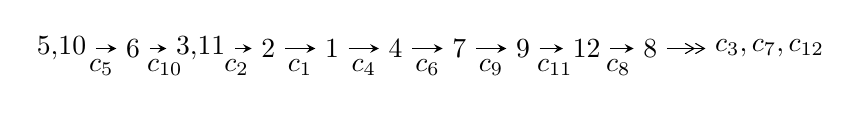
\begin{tikzpicture}[x=23pt, y=7pt]
	% node
	\node (A0) at (-1/8, 0) {5,10};
	\node (A1) at (1, 0) {6};
	\node (A2) at (33/16, 0) {3,11};
	\node (A3) at (25/8, 0) {2};
	\node (A4) at (33/8, 0) {1};
	\node (A5) at (41/8, 0) {4};
	\node (A6) at (49/8, 0) {7};
	\node (A7) at (57/8, 0) {9};
	\node (A8) at (65/8, 0) {12};
	\node (A9) at (73/8, 0) {8};
	\node (C1) at (1/2, -1) {$c_{5}$};
	\node (C2) at (3/2, -1) {$c_{10}$};
	\node (C3) at (21/8, -1) {$c_{2}$};
	\node (C4) at (29/8, -1) {$c_{1}$};
	\node (C5) at (37/8, -1) {$c_{4}$};
	\node (C6) at (45/8, -1) {$c_{6}$};
	\node (C7) at (53/8, -1) {$c_{9}$};
	\node (C8) at (61/8, -1) {$c_{11}$};
	\node (C9) at (69/8, -1) {$c_{8}$};
	\node (A10) at (11, 0) {$c_{3},c_{7},c_{12}$};

	% edge
	\draw[->,>=stealth]	
	(A0) edge (A1) (A1) edge (A2) (A2) edge (A3) (A3) edge (A4) (A4) edge (A5) (A5) edge (A6) (A6) edge (A7) (A7) edge (A8) (A8) edge (A9) ;
	\draw[->>,>={angle 60}]	
	(A9) edge (A10);
\end{tikzpicture} \\ 

\end{tabular} \\

\footnotetext{
The image of knot diagram is generated by the software ``\textbf{Draw programme}" developed by Andrew Bartholomew(\url{http://www.layer8.co.uk/maths/draw/index.htm\#Running-draw}), where we modified some parts for our purpose(\url{https://github.com/CATsTAILs/LinksPainter}).
}\phantom \\ \newline 
\centering \textbf{Ideals for irreducible components\footnotemark of $X_{\text{par}}$} 
 
\begin{align*}
I^u_{1}&=\langle 
-2.73784\times10^{105} u^{87}+2.33065\times10^{106} u^{86}+\cdots+1.32969\times10^{107} b+6.87193\times10^{107},\\
\phantom{I^u_{1}}&\phantom{= \langle  }-1.27360\times10^{106} u^{87}+7.35251\times10^{105} u^{86}+\cdots+2.65937\times10^{107} a+7.67895\times10^{107},\\
\phantom{I^u_{1}}&\phantom{= \langle  }u^{88}+2 u^{87}+\cdots+12 u-8\rangle \\
I^u_{2}&=\langle 
b+1,\;2 u^7- u^6-3 u^5+3 u^4+4 u^3-3 u^2+a-2 u+4,\;u^8- u^7- u^6+2 u^5+u^4-2 u^3+2 u-1\rangle \\
\\
I^v_{1}&=\langle 
a,\;- v^2+b-3 v+1,\;v^3+2 v^2-3 v+1\rangle \\
\end{align*}
\raggedright * 3 irreducible components of $\dim_{\mathbb{C}}=0$, with total 99 representations.\\
\footnotetext{All coefficients of polynomials are rational numbers. But the coefficients are sometimes approximated in decimal forms when there is not enough margin.}
\newpage
\renewcommand{\arraystretch}{1}
\centering \section*{I. $I^u_{1}= \langle -2.74\times10^{105} u^{87}+2.33\times10^{106} u^{86}+\cdots+1.33\times10^{107} b+6.87\times10^{107},\;-1.27\times10^{106} u^{87}+7.35\times10^{105} u^{86}+\cdots+2.66\times10^{107} a+7.68\times10^{107},\;u^{88}+2 u^{87}+\cdots+12 u-8 \rangle$}
\flushleft \textbf{(i) Arc colorings}\\
\begin{tabular}{m{7pt} m{180pt} m{7pt} m{180pt} }
\flushright $a_{5}=$&$\begin{pmatrix}1\\0\end{pmatrix}$ \\
\flushright $a_{10}=$&$\begin{pmatrix}0\\u\end{pmatrix}$ \\
\flushright $a_{6}=$&$\begin{pmatrix}1\\u^2\end{pmatrix}$ \\
\flushright $a_{3}=$&$\begin{pmatrix}0.0478909 u^{87}-0.0276475 u^{86}+\cdots+35.3569 u-2.88750\\0.0205902 u^{87}-0.175279 u^{86}+\cdots+0.764280 u-5.16808\end{pmatrix}$ \\
\flushright $a_{11}=$&$\begin{pmatrix}- u\\- u^3+u\end{pmatrix}$ \\
\flushright $a_{2}=$&$\begin{pmatrix}0.0684810 u^{87}-0.202926 u^{86}+\cdots+36.1212 u-8.05559\\0.0205902 u^{87}-0.175279 u^{86}+\cdots+0.764280 u-5.16808\end{pmatrix}$ \\
\flushright $a_{1}=$&$\begin{pmatrix}1.39916 u^{87}+3.39018 u^{86}+\cdots+13.5712 u+13.1209\\-1.39649 u^{87}-3.74999 u^{86}+\cdots-0.897228 u-18.8300\end{pmatrix}$ \\
\flushright $a_{4}=$&$\begin{pmatrix}0.408355 u^{87}+1.20087 u^{86}+\cdots+32.6967 u-0.441203\\-0.968270 u^{87}-2.08814 u^{86}+\cdots-0.974469 u-4.14421\end{pmatrix}$ \\
\flushright $a_{7}=$&$\begin{pmatrix}0.00267385 u^{87}-0.359809 u^{86}+\cdots+12.6740 u-5.70909\\1.24468 u^{87}+3.55177 u^{86}+\cdots+5.30050 u+15.9088\end{pmatrix}$ \\
\flushright $a_{9}=$&$\begin{pmatrix}u^3\\u^5- u^3+u\end{pmatrix}$ \\
\flushright $a_{12}=$&$\begin{pmatrix}- u^5- u\\- u^7+u^5-2 u^3+u\end{pmatrix}$ \\
\flushright $a_{8}=$&$\begin{pmatrix}-0.290712 u^{87}-1.73558 u^{86}+\cdots+6.94662 u-12.1213\\1.45970 u^{87}+4.30683 u^{86}+\cdots+8.54245 u+17.9540\end{pmatrix}$\\&\end{tabular}
\flushleft \textbf{(ii) Obstruction class $= -1$}\\~\\
\flushleft \textbf{(iii) Cusp Shapes $= 6.18054 u^{87}+14.8609 u^{86}+\cdots+127.311 u+12.9010$}\\~\\
\newpage\renewcommand{\arraystretch}{1}
\flushleft \textbf{(iv) u-Polynomials at the component}\newline \\
\begin{tabular}{m{50pt}|m{274pt}}
Crossings & \hspace{64pt}u-Polynomials at each crossing \\
\hline $$\begin{aligned}c_{1}\end{aligned}$$&$\begin{aligned}
&u^{88}+38 u^{87}+\cdots+101 u+1
\end{aligned}$\\
\hline $$\begin{aligned}c_{2},c_{4}\end{aligned}$$&$\begin{aligned}
&u^{88}-10 u^{87}+\cdots-7 u+1
\end{aligned}$\\
\hline $$\begin{aligned}c_{3},c_{6}\end{aligned}$$&$\begin{aligned}
&u^{88}-2 u^{87}+\cdots+128 u-256
\end{aligned}$\\
\hline $$\begin{aligned}c_{5},c_{10}\end{aligned}$$&$\begin{aligned}
&u^{88}-2 u^{87}+\cdots-12 u-8
\end{aligned}$\\
\hline $$\begin{aligned}c_{7},c_{8},c_{12}\end{aligned}$$&$\begin{aligned}
&u^{88}-5 u^{87}+\cdots+8 u+1
\end{aligned}$\\
\hline $$\begin{aligned}c_{9},c_{11}\end{aligned}$$&$\begin{aligned}
&u^{88}+24 u^{87}+\cdots+1872 u+64
\end{aligned}$\\
\hline
\end{tabular}\\~\\
\newpage\renewcommand{\arraystretch}{1}
\flushleft \textbf{(v) Riley Polynomials at the component}\newline \\
\begin{tabular}{m{50pt}|m{274pt}}
Crossings & \hspace{64pt}Riley Polynomials at each crossing \\
\hline $$\begin{aligned}c_{1}\end{aligned}$$&$\begin{aligned}
&y^{88}+34 y^{87}+\cdots-4505 y+1
\end{aligned}$\\
\hline $$\begin{aligned}c_{2},c_{4}\end{aligned}$$&$\begin{aligned}
&y^{88}-38 y^{87}+\cdots-101 y+1
\end{aligned}$\\
\hline $$\begin{aligned}c_{3},c_{6}\end{aligned}$$&$\begin{aligned}
&y^{88}+54 y^{87}+\cdots+999424 y+65536
\end{aligned}$\\
\hline $$\begin{aligned}c_{5},c_{10}\end{aligned}$$&$\begin{aligned}
&y^{88}-24 y^{87}+\cdots-1872 y+64
\end{aligned}$\\
\hline $$\begin{aligned}c_{7},c_{8},c_{12}\end{aligned}$$&$\begin{aligned}
&y^{88}-71 y^{87}+\cdots+62 y+1
\end{aligned}$\\
\hline $$\begin{aligned}c_{9},c_{11}\end{aligned}$$&$\begin{aligned}
&y^{88}+76 y^{87}+\cdots-105728 y+4096
\end{aligned}$\\
\hline
\end{tabular}\\~\\
\newpage\flushleft \textbf{(vi) Complex Volumes and Cusp Shapes}
$$\begin{array}{c|c|c}  
\text{Solutions to }I^u_{1}& \I (\text{vol} + \sqrt{-1}CS) & \text{Cusp shape}\\
 \hline 
\begin{aligned}
u &= \phantom{-}0.392572 + 0.920696 I \\
a &= \phantom{-}0.031296 - 0.890953 I \\
b &= \phantom{-}0.670708 + 0.469662 I\end{aligned}
 & -1.30721 + 0.66243 I & \phantom{-0.000000 } 0 \\ \hline\begin{aligned}
u &= \phantom{-}0.392572 - 0.920696 I \\
a &= \phantom{-}0.031296 + 0.890953 I \\
b &= \phantom{-}0.670708 - 0.469662 I\end{aligned}
 & -1.30721 - 0.66243 I & \phantom{-0.000000 } 0 \\ \hline\begin{aligned}
u &= -0.887881 + 0.457891 I \\
a &= -0.090976 + 0.352185 I \\
b &= \phantom{-}0.479587 + 0.533093 I\end{aligned}
 & \phantom{-}1.43432 + 2.39937 I & \phantom{-0.000000 } 0 \\ \hline\begin{aligned}
u &= -0.887881 - 0.457891 I \\
a &= -0.090976 - 0.352185 I \\
b &= \phantom{-}0.479587 - 0.533093 I\end{aligned}
 & \phantom{-}1.43432 - 2.39937 I & \phantom{-0.000000 } 0 \\ \hline\begin{aligned}
u &= \phantom{-}0.203330 + 1.003580 I \\
a &= -0.381810 + 0.869323 I \\
b &= \phantom{-}0.991760 - 0.565904 I\end{aligned}
 & -2.39788 + 5.04856 I & \phantom{-0.000000 } 0 \\ \hline\begin{aligned}
u &= \phantom{-}0.203330 - 1.003580 I \\
a &= -0.381810 - 0.869323 I \\
b &= \phantom{-}0.991760 + 0.565904 I\end{aligned}
 & -2.39788 - 5.04856 I & \phantom{-0.000000 } 0 \\ \hline\begin{aligned}
u &= -0.958732 + 0.139931 I \\
a &= \phantom{-}0.735606 + 0.670342 I \\
b &= -0.335372 - 0.551660 I\end{aligned}
 & -5.40258 + 0.56073 I & \phantom{-0.000000 } 0 \\ \hline\begin{aligned}
u &= -0.958732 - 0.139931 I \\
a &= \phantom{-}0.735606 - 0.670342 I \\
b &= -0.335372 + 0.551660 I\end{aligned}
 & -5.40258 - 0.56073 I & \phantom{-0.000000 } 0 \\ \hline\begin{aligned}
u &= -0.862313 + 0.579468 I \\
a &= \phantom{-}0.321746 + 0.371790 I \\
b &= \phantom{-}0.515120 + 0.203414 I\end{aligned}
 & \phantom{-}1.47628 + 2.33295 I & \phantom{-0.000000 } 0 \\ \hline\begin{aligned}
u &= -0.862313 - 0.579468 I \\
a &= \phantom{-}0.321746 - 0.371790 I \\
b &= \phantom{-}0.515120 - 0.203414 I\end{aligned}
 & \phantom{-}1.47628 - 2.33295 I & \phantom{-0.000000 } 0\\
 \hline 
 \end{array}$$\newpage$$\begin{array}{c|c|c}  
\text{Solutions to }I^u_{1}& \I (\text{vol} + \sqrt{-1}CS) & \text{Cusp shape}\\
 \hline 
\begin{aligned}
u &= \phantom{-}0.947226 + 0.084231 I \\
a &= \phantom{-}1.94827 - 0.02918 I \\
b &= \phantom{-}0.941810 + 0.560456 I\end{aligned}
 & -0.97747 - 2.78041 I & -12.00000 + 0. I\phantom{ +0.000000I} \\ \hline\begin{aligned}
u &= \phantom{-}0.947226 - 0.084231 I \\
a &= \phantom{-}1.94827 + 0.02918 I \\
b &= \phantom{-}0.941810 - 0.560456 I\end{aligned}
 & -0.97747 + 2.78041 I & -12.00000 + 0. I\phantom{ +0.000000I} \\ \hline\begin{aligned}
u &= -1.000340 + 0.317524 I \\
a &= \phantom{-}1.70909 + 1.08359 I \\
b &= \phantom{-}1.024730 - 0.591282 I\end{aligned}
 & -0.03297 + 7.08755 I & \phantom{-0.000000 } 0 \\ \hline\begin{aligned}
u &= -1.000340 - 0.317524 I \\
a &= \phantom{-}1.70909 - 1.08359 I \\
b &= \phantom{-}1.024730 + 0.591282 I\end{aligned}
 & -0.03297 - 7.08755 I & \phantom{-0.000000 } 0 \\ \hline\begin{aligned}
u &= \phantom{-}1.044510 + 0.227043 I \\
a &= -0.930430 - 0.232517 I \\
b &= -1.224440 + 0.244106 I\end{aligned}
 & -8.09834 - 2.07994 I & \phantom{-0.000000 } 0 \\ \hline\begin{aligned}
u &= \phantom{-}1.044510 - 0.227043 I \\
a &= -0.930430 + 0.232517 I \\
b &= -1.224440 - 0.244106 I\end{aligned}
 & -8.09834 + 2.07994 I & \phantom{-0.000000 } 0 \\ \hline\begin{aligned}
u &= \phantom{-}0.870126 + 0.281441 I \\
a &= \phantom{-}0.615716 - 1.177220 I \\
b &= \phantom{-}0.759307 - 0.539626 I\end{aligned}
 & -0.37405 + 1.65782 I & -12.00000 + 0. I\phantom{ +0.000000I} \\ \hline\begin{aligned}
u &= \phantom{-}0.870126 - 0.281441 I \\
a &= \phantom{-}0.615716 + 1.177220 I \\
b &= \phantom{-}0.759307 + 0.539626 I\end{aligned}
 & -0.37405 - 1.65782 I & -12.00000 + 0. I\phantom{ +0.000000I} \\ \hline\begin{aligned}
u &= -1.058740 + 0.305027 I \\
a &= -0.70456 - 1.67547 I \\
b &= -1.073140 + 0.441465 I\end{aligned}
 & -7.60787 + 4.58396 I & \phantom{-0.000000 } 0 \\ \hline\begin{aligned}
u &= -1.058740 - 0.305027 I \\
a &= -0.70456 + 1.67547 I \\
b &= -1.073140 - 0.441465 I\end{aligned}
 & -7.60787 - 4.58396 I & \phantom{-0.000000 } 0\\
 \hline 
 \end{array}$$\newpage$$\begin{array}{c|c|c}  
\text{Solutions to }I^u_{1}& \I (\text{vol} + \sqrt{-1}CS) & \text{Cusp shape}\\
 \hline 
\begin{aligned}
u &= -0.753149 + 0.812851 I \\
a &= \phantom{-}0.009896 - 1.120230 I \\
b &= -1.306960 + 0.017227 I\end{aligned}
 & -1.25565 - 1.36378 I & \phantom{-0.000000 } 0 \\ \hline\begin{aligned}
u &= -0.753149 - 0.812851 I \\
a &= \phantom{-}0.009896 + 1.120230 I \\
b &= -1.306960 - 0.017227 I\end{aligned}
 & -1.25565 + 1.36378 I & \phantom{-0.000000 } 0 \\ \hline\begin{aligned}
u &= \phantom{-}1.038570 + 0.425588 I \\
a &= -0.126062 + 0.339240 I \\
b &= \phantom{-}0.227675 - 0.708873 I\end{aligned}
 & -3.58769 - 5.33790 I & \phantom{-0.000000 } 0 \\ \hline\begin{aligned}
u &= \phantom{-}1.038570 - 0.425588 I \\
a &= -0.126062 - 0.339240 I \\
b &= \phantom{-}0.227675 + 0.708873 I\end{aligned}
 & -3.58769 + 5.33790 I & \phantom{-0.000000 } 0 \\ \hline\begin{aligned}
u &= -0.822672 + 0.764737 I \\
a &= -0.560044 - 1.062490 I \\
b &= \phantom{-}1.088910 + 0.759677 I\end{aligned}
 & \phantom{-}4.24766 - 1.27868 I & \phantom{-0.000000 } 0 \\ \hline\begin{aligned}
u &= -0.822672 - 0.764737 I \\
a &= -0.560044 + 1.062490 I \\
b &= \phantom{-}1.088910 - 0.759677 I\end{aligned}
 & \phantom{-}4.24766 + 1.27868 I & \phantom{-0.000000 } 0 \\ \hline\begin{aligned}
u &= \phantom{-}0.814865 + 0.778282 I \\
a &= \phantom{-}0.11774 + 2.41231 I \\
b &= -0.830940 - 0.592246 I\end{aligned}
 & \phantom{-}0.329058 - 0.951263 I & \phantom{-0.000000 } 0 \\ \hline\begin{aligned}
u &= \phantom{-}0.814865 - 0.778282 I \\
a &= \phantom{-}0.11774 - 2.41231 I \\
b &= -0.830940 + 0.592246 I\end{aligned}
 & \phantom{-}0.329058 + 0.951263 I & \phantom{-0.000000 } 0 \\ \hline\begin{aligned}
u &= \phantom{-}0.754800 + 0.876512 I \\
a &= \phantom{-}1.11868 - 1.17948 I \\
b &= -0.868291 + 0.595565 I\end{aligned}
 & \phantom{-}0.20885 + 3.75440 I & \phantom{-0.000000 } 0 \\ \hline\begin{aligned}
u &= \phantom{-}0.754800 - 0.876512 I \\
a &= \phantom{-}1.11868 + 1.17948 I \\
b &= -0.868291 - 0.595565 I\end{aligned}
 & \phantom{-}0.20885 - 3.75440 I & \phantom{-0.000000 } 0\\
 \hline 
 \end{array}$$\newpage$$\begin{array}{c|c|c}  
\text{Solutions to }I^u_{1}& \I (\text{vol} + \sqrt{-1}CS) & \text{Cusp shape}\\
 \hline 
\begin{aligned}
u &= \phantom{-}0.794082 + 0.262125 I \\
a &= -1.46161 + 2.25876 I \\
b &= -0.977760 - 0.341426 I\end{aligned}
 & -2.28886 - 2.45162 I & -16.2110 + 6.3903 I \\ \hline\begin{aligned}
u &= \phantom{-}0.794082 - 0.262125 I \\
a &= -1.46161 - 2.25876 I \\
b &= -0.977760 + 0.341426 I\end{aligned}
 & -2.28886 + 2.45162 I & -16.2110 - 6.3903 I \\ \hline\begin{aligned}
u &= -0.852305 + 0.811962 I \\
a &= \phantom{-}1.07072 + 1.14717 I \\
b &= -0.811618 - 0.630399 I\end{aligned}
 & \phantom{-}4.01818 + 0.54192 I & \phantom{-0.000000 } 0 \\ \hline\begin{aligned}
u &= -0.852305 - 0.811962 I \\
a &= \phantom{-}1.07072 - 1.14717 I \\
b &= -0.811618 + 0.630399 I\end{aligned}
 & \phantom{-}4.01818 - 0.54192 I & \phantom{-0.000000 } 0 \\ \hline\begin{aligned}
u &= \phantom{-}0.886190 + 0.782136 I \\
a &= -0.057066 + 0.858549 I \\
b &= -1.336480 + 0.029864 I\end{aligned}
 & \phantom{-}2.31687 - 2.94399 I & \phantom{-0.000000 } 0 \\ \hline\begin{aligned}
u &= \phantom{-}0.886190 - 0.782136 I \\
a &= -0.057066 - 0.858549 I \\
b &= -1.336480 - 0.029864 I\end{aligned}
 & \phantom{-}2.31687 + 2.94399 I & \phantom{-0.000000 } 0 \\ \hline\begin{aligned}
u &= \phantom{-}0.790264 + 0.884911 I \\
a &= -0.576247 + 1.018820 I \\
b &= \phantom{-}1.111540 - 0.727657 I\end{aligned}
 & \phantom{-}7.85733 + 5.61860 I & \phantom{-0.000000 } 0 \\ \hline\begin{aligned}
u &= \phantom{-}0.790264 - 0.884911 I \\
a &= -0.576247 - 1.018820 I \\
b &= \phantom{-}1.111540 + 0.727657 I\end{aligned}
 & \phantom{-}7.85733 - 5.61860 I & \phantom{-0.000000 } 0 \\ \hline\begin{aligned}
u &= -0.881857 + 0.797266 I \\
a &= -0.10968 + 1.44896 I \\
b &= \phantom{-}0.605815 - 0.957019 I\end{aligned}
 & \phantom{-}5.72724 + 4.97749 I & \phantom{-0.000000 } 0 \\ \hline\begin{aligned}
u &= -0.881857 - 0.797266 I \\
a &= -0.10968 - 1.44896 I \\
b &= \phantom{-}0.605815 + 0.957019 I\end{aligned}
 & \phantom{-}5.72724 - 4.97749 I & \phantom{-0.000000 } 0\\
 \hline 
 \end{array}$$\newpage$$\begin{array}{c|c|c}  
\text{Solutions to }I^u_{1}& \I (\text{vol} + \sqrt{-1}CS) & \text{Cusp shape}\\
 \hline 
\begin{aligned}
u &= -0.933371 + 0.742677 I \\
a &= \phantom{-}0.74662 + 2.29509 I \\
b &= \phantom{-}1.113350 - 0.705726 I\end{aligned}
 & \phantom{-}3.90440 + 6.99279 I & \phantom{-0.000000 } 0 \\ \hline\begin{aligned}
u &= -0.933371 - 0.742677 I \\
a &= \phantom{-}0.74662 - 2.29509 I \\
b &= \phantom{-}1.113350 + 0.705726 I\end{aligned}
 & \phantom{-}3.90440 - 6.99279 I & \phantom{-0.000000 } 0 \\ \hline\begin{aligned}
u &= -0.897183 + 0.796476 I \\
a &= -1.216610 - 0.564361 I \\
b &= \phantom{-}0.532139 + 0.928269 I\end{aligned}
 & \phantom{-}5.68216 + 1.00101 I & \phantom{-0.000000 } 0 \\ \hline\begin{aligned}
u &= -0.897183 - 0.796476 I \\
a &= -1.216610 + 0.564361 I \\
b &= \phantom{-}0.532139 - 0.928269 I\end{aligned}
 & \phantom{-}5.68216 - 1.00101 I & \phantom{-0.000000 } 0 \\ \hline\begin{aligned}
u &= \phantom{-}0.942078 + 0.752491 I \\
a &= \phantom{-}1.01680 - 1.12508 I \\
b &= -0.759566 + 0.665808 I\end{aligned}
 & -0.06234 - 4.83478 I & \phantom{-0.000000 } 0 \\ \hline\begin{aligned}
u &= \phantom{-}0.942078 - 0.752491 I \\
a &= \phantom{-}1.01680 + 1.12508 I \\
b &= -0.759566 - 0.665808 I\end{aligned}
 & -0.06234 + 4.83478 I & \phantom{-0.000000 } 0 \\ \hline\begin{aligned}
u &= \phantom{-}0.422280 + 0.670799 I \\
a &= \phantom{-}0.704032 - 0.641404 I \\
b &= \phantom{-}0.214950 + 0.166258 I\end{aligned}
 & -1.40337 + 0.92720 I & -8.23175 - 0.58902 I \\ \hline\begin{aligned}
u &= \phantom{-}0.422280 - 0.670799 I \\
a &= \phantom{-}0.704032 + 0.641404 I \\
b &= \phantom{-}0.214950 - 0.166258 I\end{aligned}
 & -1.40337 - 0.92720 I & -8.23175 + 0.58902 I \\ \hline\begin{aligned}
u &= \phantom{-}0.841271 + 0.874220 I \\
a &= -0.05629 - 1.46245 I \\
b &= \phantom{-}0.555731 + 0.949544 I\end{aligned}
 & \phantom{-}9.56149 - 0.50937 I & \phantom{-0.000000 } 0 \\ \hline\begin{aligned}
u &= \phantom{-}0.841271 - 0.874220 I \\
a &= -0.05629 + 1.46245 I \\
b &= \phantom{-}0.555731 - 0.949544 I\end{aligned}
 & \phantom{-}9.56149 + 0.50937 I & \phantom{-0.000000 } 0\\
 \hline 
 \end{array}$$\newpage$$\begin{array}{c|c|c}  
\text{Solutions to }I^u_{1}& \I (\text{vol} + \sqrt{-1}CS) & \text{Cusp shape}\\
 \hline 
\begin{aligned}
u &= -0.925474 + 0.790304 I \\
a &= \phantom{-}0.08043 - 2.24661 I \\
b &= -0.884202 + 0.625072 I\end{aligned}
 & \phantom{-}3.79156 + 5.46140 I & \phantom{-0.000000 } 0 \\ \hline\begin{aligned}
u &= -0.925474 - 0.790304 I \\
a &= \phantom{-}0.08043 + 2.24661 I \\
b &= -0.884202 - 0.625072 I\end{aligned}
 & \phantom{-}3.79156 - 5.46140 I & \phantom{-0.000000 } 0 \\ \hline\begin{aligned}
u &= -1.220990 + 0.093727 I \\
a &= \phantom{-}0.893667 + 0.033167 I \\
b &= \phantom{-}0.943866 + 0.417931 I\end{aligned}
 & -7.95540 - 1.57335 I & \phantom{-0.000000 } 0 \\ \hline\begin{aligned}
u &= -1.220990 - 0.093727 I \\
a &= \phantom{-}0.893667 - 0.033167 I \\
b &= \phantom{-}0.943866 - 0.417931 I\end{aligned}
 & -7.95540 + 1.57335 I & \phantom{-0.000000 } 0 \\ \hline\begin{aligned}
u &= -0.794180 + 0.936665 I \\
a &= -0.00264 + 1.47095 I \\
b &= \phantom{-}0.507424 - 0.936810 I\end{aligned}
 & \phantom{-}5.50773 - 3.95377 I & \phantom{-0.000000 } 0 \\ \hline\begin{aligned}
u &= -0.794180 - 0.936665 I \\
a &= -0.00264 - 1.47095 I \\
b &= \phantom{-}0.507424 + 0.936810 I\end{aligned}
 & \phantom{-}5.50773 + 3.95377 I & \phantom{-0.000000 } 0 \\ \hline\begin{aligned}
u &= -0.088205 + 0.759173 I \\
a &= \phantom{-}1.39479 + 1.62378 I \\
b &= -1.025110 - 0.260624 I\end{aligned}
 & -4.33853 - 0.93069 I & -17.4874 - 0.5005 I \\ \hline\begin{aligned}
u &= -0.088205 - 0.759173 I \\
a &= \phantom{-}1.39479 - 1.62378 I \\
b &= -1.025110 + 0.260624 I\end{aligned}
 & -4.33853 + 0.93069 I & -17.4874 + 0.5005 I \\ \hline\begin{aligned}
u &= -0.758355 + 0.979789 I \\
a &= -0.587135 - 0.981162 I \\
b &= \phantom{-}1.128270 + 0.699547 I\end{aligned}
 & \phantom{-}3.60923 - 9.94654 I & \phantom{-0.000000 } 0 \\ \hline\begin{aligned}
u &= -0.758355 - 0.979789 I \\
a &= -0.587135 + 0.981162 I \\
b &= \phantom{-}1.128270 - 0.699547 I\end{aligned}
 & \phantom{-}3.60923 + 9.94654 I & \phantom{-0.000000 } 0\\
 \hline 
 \end{array}$$\newpage$$\begin{array}{c|c|c}  
\text{Solutions to }I^u_{1}& \I (\text{vol} + \sqrt{-1}CS) & \text{Cusp shape}\\
 \hline 
\begin{aligned}
u &= -0.985719 + 0.755243 I \\
a &= -0.071592 - 0.666243 I \\
b &= -1.357700 - 0.065878 I\end{aligned}
 & -1.95959 + 7.25560 I & \phantom{-0.000000 } 0 \\ \hline\begin{aligned}
u &= -0.985719 - 0.755243 I \\
a &= -0.071592 + 0.666243 I \\
b &= -1.357700 + 0.065878 I\end{aligned}
 & -1.95959 - 7.25560 I & \phantom{-0.000000 } 0 \\ \hline\begin{aligned}
u &= \phantom{-}1.180680 + 0.413243 I \\
a &= \phantom{-}1.03880 - 1.13972 I \\
b &= \phantom{-}1.094140 + 0.563802 I\end{aligned}
 & -5.89137 - 10.06180 I & \phantom{-0.000000 } 0 \\ \hline\begin{aligned}
u &= \phantom{-}1.180680 - 0.413243 I \\
a &= \phantom{-}1.03880 + 1.13972 I \\
b &= \phantom{-}1.094140 - 0.563802 I\end{aligned}
 & -5.89137 + 10.06180 I & \phantom{-0.000000 } 0 \\ \hline\begin{aligned}
u &= \phantom{-}1.078160 + 0.638701 I \\
a &= \phantom{-}0.332709 - 0.353621 I \\
b &= \phantom{-}0.716392 - 0.192203 I\end{aligned}
 & -3.33914 - 6.07366 I & \phantom{-0.000000 } 0 \\ \hline\begin{aligned}
u &= \phantom{-}1.078160 - 0.638701 I \\
a &= \phantom{-}0.332709 + 0.353621 I \\
b &= \phantom{-}0.716392 + 0.192203 I\end{aligned}
 & -3.33914 + 6.07366 I & \phantom{-0.000000 } 0 \\ \hline\begin{aligned}
u &= -0.365420 + 0.646101 I \\
a &= -0.146644 + 1.102250 I \\
b &= \phantom{-}0.746131 - 0.685305 I\end{aligned}
 & \phantom{-}3.13319 + 1.58793 I & -4.36565 - 2.62454 I \\ \hline\begin{aligned}
u &= -0.365420 - 0.646101 I \\
a &= -0.146644 - 1.102250 I \\
b &= \phantom{-}0.746131 + 0.685305 I\end{aligned}
 & \phantom{-}3.13319 - 1.58793 I & -4.36565 + 2.62454 I \\ \hline\begin{aligned}
u &= \phantom{-}0.963850 + 0.822645 I \\
a &= -1.090440 + 0.696675 I \\
b &= \phantom{-}0.499212 - 0.961407 I\end{aligned}
 & \phantom{-}9.17313 - 5.78375 I & \phantom{-0.000000 } 0 \\ \hline\begin{aligned}
u &= \phantom{-}0.963850 - 0.822645 I \\
a &= -1.090440 - 0.696675 I \\
b &= \phantom{-}0.499212 + 0.961407 I\end{aligned}
 & \phantom{-}9.17313 + 5.78375 I & \phantom{-0.000000 } 0\\
 \hline 
 \end{array}$$\newpage$$\begin{array}{c|c|c}  
\text{Solutions to }I^u_{1}& \I (\text{vol} + \sqrt{-1}CS) & \text{Cusp shape}\\
 \hline 
\begin{aligned}
u &= -0.710725 + 0.142036 I \\
a &= -2.49015 - 0.07252 I \\
b &= -1.090730 - 0.165721 I\end{aligned}
 & -2.74417 + 0.55471 I & -16.6137 - 8.8786 I \\ \hline\begin{aligned}
u &= -0.710725 - 0.142036 I \\
a &= -2.49015 + 0.07252 I \\
b &= -1.090730 + 0.165721 I\end{aligned}
 & -2.74417 - 0.55471 I & -16.6137 + 8.8786 I \\ \hline\begin{aligned}
u &= \phantom{-}1.008330 + 0.782072 I \\
a &= \phantom{-}0.05748 + 2.13739 I \\
b &= -0.926480 - 0.640157 I\end{aligned}
 & -0.57700 - 9.90939 I & \phantom{-0.000000 } 0 \\ \hline\begin{aligned}
u &= \phantom{-}1.008330 - 0.782072 I \\
a &= \phantom{-}0.05748 - 2.13739 I \\
b &= -0.926480 + 0.640157 I\end{aligned}
 & -0.57700 + 9.90939 I & \phantom{-0.000000 } 0 \\ \hline\begin{aligned}
u &= \phantom{-}0.998606 + 0.799996 I \\
a &= \phantom{-}0.54095 - 2.15791 I \\
b &= \phantom{-}1.142060 + 0.706012 I\end{aligned}
 & \phantom{-}7.20070 - 11.86680 I & \phantom{-0.000000 } 0 \\ \hline\begin{aligned}
u &= \phantom{-}0.998606 - 0.799996 I \\
a &= \phantom{-}0.54095 + 2.15791 I \\
b &= \phantom{-}1.142060 - 0.706012 I\end{aligned}
 & \phantom{-}7.20070 + 11.86680 I & \phantom{-0.000000 } 0 \\ \hline\begin{aligned}
u &= -1.021860 + 0.824555 I \\
a &= -0.979873 - 0.762766 I \\
b &= \phantom{-}0.466549 + 0.980590 I\end{aligned}
 & \phantom{-}4.77490 + 10.43370 I & \phantom{-0.000000 } 0 \\ \hline\begin{aligned}
u &= -1.021860 - 0.824555 I \\
a &= -0.979873 + 0.762766 I \\
b &= \phantom{-}0.466549 - 0.980590 I\end{aligned}
 & \phantom{-}4.77490 - 10.43370 I & \phantom{-0.000000 } 0 \\ \hline\begin{aligned}
u &= -0.199533 + 0.630090 I \\
a &= -0.349695 - 1.014370 I \\
b &= \phantom{-}0.931055 + 0.671220 I\end{aligned}
 & \phantom{-}2.58372 - 3.65091 I & -4.88024 + 4.09202 I \\ \hline\begin{aligned}
u &= -0.199533 - 0.630090 I \\
a &= -0.349695 + 1.014370 I \\
b &= \phantom{-}0.931055 - 0.671220 I\end{aligned}
 & \phantom{-}2.58372 + 3.65091 I & -4.88024 - 4.09202 I\\
 \hline 
 \end{array}$$\newpage$$\begin{array}{c|c|c}  
\text{Solutions to }I^u_{1}& \I (\text{vol} + \sqrt{-1}CS) & \text{Cusp shape}\\
 \hline 
\begin{aligned}
u &= -1.059800 + 0.822621 I \\
a &= \phantom{-}0.44539 + 2.02899 I \\
b &= \phantom{-}1.162810 - 0.698617 I\end{aligned}
 & \phantom{-}2.6344 + 16.5403 I & \phantom{-0.000000 } 0 \\ \hline\begin{aligned}
u &= -1.059800 - 0.822621 I \\
a &= \phantom{-}0.44539 - 2.02899 I \\
b &= \phantom{-}1.162810 + 0.698617 I\end{aligned}
 & \phantom{-}2.6344 - 16.5403 I & \phantom{-0.000000 } 0 \\ \hline\begin{aligned}
u &= \phantom{-}0.646965 + 0.080521 I \\
a &= -0.343025 - 1.213620 I \\
b &= \phantom{-}0.873530 + 0.830831 I\end{aligned}
 & \phantom{-}0.75119 - 3.07502 I & -19.2370 + 4.9728 I \\ \hline\begin{aligned}
u &= \phantom{-}0.646965 - 0.080521 I \\
a &= -0.343025 + 1.213620 I \\
b &= \phantom{-}0.873530 - 0.830831 I\end{aligned}
 & \phantom{-}0.75119 + 3.07502 I & -19.2370 - 4.9728 I \\ \hline\begin{aligned}
u &= \phantom{-}0.549522\phantom{ +0.000000I} \\
a &= \phantom{-}0.875721\phantom{ +0.000000I} \\
b &= -0.119846\phantom{ +0.000000I}\end{aligned}
 & -0.718836\phantom{ +0.000000I} & -14.1050\phantom{ +0.000000I} \\ \hline\begin{aligned}
u &= \phantom{-}0.317305 + 0.268219 I \\
a &= \phantom{-}1.79149 - 0.55439 I \\
b &= -0.724370 + 0.147571 I\end{aligned}
 & -0.979988 + 0.105759 I & -9.79769 + 1.06695 I \\ \hline\begin{aligned}
u &= \phantom{-}0.317305 - 0.268219 I \\
a &= \phantom{-}1.79149 + 0.55439 I \\
b &= -0.724370 - 0.147571 I\end{aligned}
 & -0.979988 - 0.105759 I & -9.79769 - 1.06695 I \\ \hline\begin{aligned}
u &= -0.344030\phantom{ +0.000000I} \\
a &= -11.6544\phantom{ +0.000000I} \\
b &= -0.902968\phantom{ +0.000000I}\end{aligned}
 & -2.97247\phantom{ +0.000000I} & -58.0340\phantom{ +0.000000I}\\
 \hline 
 \end{array}$$\newpage\newpage\renewcommand{\arraystretch}{1}
\centering \section*{II. $I^u_{2}= \langle b+1,\;2 u^7- u^6-3 u^5+3 u^4+4 u^3-3 u^2+a-2 u+4,\;u^8- u^7- u^6+2 u^5+u^4-2 u^3+2 u-1 \rangle$}
\flushleft \textbf{(i) Arc colorings}\\
\begin{tabular}{m{7pt} m{180pt} m{7pt} m{180pt} }
\flushright $a_{5}=$&$\begin{pmatrix}1\\0\end{pmatrix}$ \\
\flushright $a_{10}=$&$\begin{pmatrix}0\\u\end{pmatrix}$ \\
\flushright $a_{6}=$&$\begin{pmatrix}1\\u^2\end{pmatrix}$ \\
\flushright $a_{3}=$&$\begin{pmatrix}-2 u^7+u^6+3 u^5-3 u^4-4 u^3+3 u^2+2 u-4\\-1\end{pmatrix}$ \\
\flushright $a_{11}=$&$\begin{pmatrix}- u\\- u^3+u\end{pmatrix}$ \\
\flushright $a_{2}=$&$\begin{pmatrix}-2 u^7+u^6+3 u^5-3 u^4-4 u^3+3 u^2+2 u-5\\-1\end{pmatrix}$ \\
\flushright $a_{1}=$&$\begin{pmatrix}-1\\0\end{pmatrix}$ \\
\flushright $a_{4}=$&$\begin{pmatrix}-2 u^7+u^6+3 u^5-3 u^4-4 u^3+3 u^2+2 u-4\\-1\end{pmatrix}$ \\
\flushright $a_{7}=$&$\begin{pmatrix}1\\u^2\end{pmatrix}$ \\
\flushright $a_{9}=$&$\begin{pmatrix}u^3\\u^5- u^3+u\end{pmatrix}$ \\
\flushright $a_{12}=$&$\begin{pmatrix}- u^5- u\\- u^7+u^5-2 u^3+u\end{pmatrix}$ \\
\flushright $a_{8}=$&$\begin{pmatrix}u^5+u\\u^5- u^3+u\end{pmatrix}$\\&\end{tabular}
\flushleft \textbf{(ii) Obstruction class $= 1$}\\~\\
\flushleft \textbf{(iii) Cusp Shapes $= 2 u^7-2 u^6+4 u^4+3 u^3- u^2-13$}\\~\\
\newpage\renewcommand{\arraystretch}{1}
\flushleft \textbf{(iv) u-Polynomials at the component}\newline \\
\begin{tabular}{m{50pt}|m{274pt}}
Crossings & \hspace{64pt}u-Polynomials at each crossing \\
\hline $$\begin{aligned}c_{1},c_{2}\end{aligned}$$&$\begin{aligned}
&(u-1)^8
\end{aligned}$\\
\hline $$\begin{aligned}c_{3},c_{6}\end{aligned}$$&$\begin{aligned}
&u^8
\end{aligned}$\\
\hline $$\begin{aligned}c_{4}\end{aligned}$$&$\begin{aligned}
&(u+1)^8
\end{aligned}$\\
\hline $$\begin{aligned}c_{5}\end{aligned}$$&$\begin{aligned}
&u^8- u^7- u^6+2 u^5+u^4-2 u^3+2 u-1
\end{aligned}$\\
\hline $$\begin{aligned}c_{7},c_{8}\end{aligned}$$&$\begin{aligned}
&u^8+u^7-3 u^6-2 u^5+3 u^4+2 u-1
\end{aligned}$\\
\hline $$\begin{aligned}c_{9}\end{aligned}$$&$\begin{aligned}
&u^8-3 u^7+7 u^6-10 u^5+11 u^4-10 u^3+6 u^2-4 u+1
\end{aligned}$\\
\hline $$\begin{aligned}c_{10}\end{aligned}$$&$\begin{aligned}
&u^8+u^7- u^6-2 u^5+u^4+2 u^3-2 u-1
\end{aligned}$\\
\hline $$\begin{aligned}c_{11}\end{aligned}$$&$\begin{aligned}
&u^8+3 u^7+7 u^6+10 u^5+11 u^4+10 u^3+6 u^2+4 u+1
\end{aligned}$\\
\hline $$\begin{aligned}c_{12}\end{aligned}$$&$\begin{aligned}
&u^8- u^7-3 u^6+2 u^5+3 u^4-2 u-1
\end{aligned}$\\
\hline
\end{tabular}\\~\\
\newpage\renewcommand{\arraystretch}{1}
\flushleft \textbf{(v) Riley Polynomials at the component}\newline \\
\begin{tabular}{m{50pt}|m{274pt}}
Crossings & \hspace{64pt}Riley Polynomials at each crossing \\
\hline $$\begin{aligned}c_{1},c_{2},c_{4}\end{aligned}$$&$\begin{aligned}
&(y-1)^8
\end{aligned}$\\
\hline $$\begin{aligned}c_{3},c_{6}\end{aligned}$$&$\begin{aligned}
&y^8
\end{aligned}$\\
\hline $$\begin{aligned}c_{5},c_{10}\end{aligned}$$&$\begin{aligned}
&y^8-3 y^7+7 y^6-10 y^5+11 y^4-10 y^3+6 y^2-4 y+1
\end{aligned}$\\
\hline $$\begin{aligned}c_{7},c_{8},c_{12}\end{aligned}$$&$\begin{aligned}
&y^8-7 y^7+19 y^6-22 y^5+3 y^4+14 y^3-6 y^2-4 y+1
\end{aligned}$\\
\hline $$\begin{aligned}c_{9},c_{11}\end{aligned}$$&$\begin{aligned}
&y^8+5 y^7+11 y^6+6 y^5-17 y^4-34 y^3-22 y^2-4 y+1
\end{aligned}$\\
\hline
\end{tabular}\\~\\
\newpage\flushleft \textbf{(vi) Complex Volumes and Cusp Shapes}
$$\begin{array}{c|c|c}  
\text{Solutions to }I^u_{2}& \I (\text{vol} + \sqrt{-1}CS) & \text{Cusp shape}\\
 \hline 
\begin{aligned}
u &= \phantom{-}0.570868 + 0.730671 I \\
a &= \phantom{-}0.281371 + 1.128550 I \\
b &= -1.00000\phantom{ +0.000000I}\end{aligned}
 & -2.68559 + 1.13123 I & -17.2624 - 0.2227 I \\ \hline\begin{aligned}
u &= \phantom{-}0.570868 - 0.730671 I \\
a &= \phantom{-}0.281371 - 1.128550 I \\
b &= -1.00000\phantom{ +0.000000I}\end{aligned}
 & -2.68559 - 1.13123 I & -17.2624 + 0.2227 I \\ \hline\begin{aligned}
u &= -0.855237 + 0.665892 I \\
a &= -0.208670 - 0.825203 I \\
b &= -1.00000\phantom{ +0.000000I}\end{aligned}
 & \phantom{-}0.51448 + 2.57849 I & -14.1288 - 3.8797 I \\ \hline\begin{aligned}
u &= -0.855237 - 0.665892 I \\
a &= -0.208670 + 0.825203 I \\
b &= -1.00000\phantom{ +0.000000I}\end{aligned}
 & \phantom{-}0.51448 - 2.57849 I & -14.1288 + 3.8797 I \\ \hline\begin{aligned}
u &= -1.09818\phantom{ +0.000000I} \\
a &= -0.829189\phantom{ +0.000000I} \\
b &= -1.00000\phantom{ +0.000000I}\end{aligned}
 & -8.14766\phantom{ +0.000000I} & -19.7220\phantom{ +0.000000I} \\ \hline\begin{aligned}
u &= \phantom{-}1.031810 + 0.655470 I \\
a &= -0.284386 + 0.605794 I \\
b &= -1.00000\phantom{ +0.000000I}\end{aligned}
 & -4.02461 - 6.44354 I & -19.1410 + 6.6674 I \\ \hline\begin{aligned}
u &= \phantom{-}1.031810 - 0.655470 I \\
a &= -0.284386 - 0.605794 I \\
b &= -1.00000\phantom{ +0.000000I}\end{aligned}
 & -4.02461 + 6.44354 I & -19.1410 - 6.6674 I \\ \hline\begin{aligned}
u &= \phantom{-}0.603304\phantom{ +0.000000I} \\
a &= -2.74744\phantom{ +0.000000I} \\
b &= -1.00000\phantom{ +0.000000I}\end{aligned}
 & -2.48997\phantom{ +0.000000I} & -12.2140\phantom{ +0.000000I}\\
 \hline 
 \end{array}$$\newpage\newpage\renewcommand{\arraystretch}{1}
\centering \section*{III. $I^v_{1}= \langle a,\;- v^2+b-3 v+1,\;v^3+2 v^2-3 v+1 \rangle$}
\flushleft \textbf{(i) Arc colorings}\\
\begin{tabular}{m{7pt} m{180pt} m{7pt} m{180pt} }
\flushright $a_{5}=$&$\begin{pmatrix}1\\0\end{pmatrix}$ \\
\flushright $a_{10}=$&$\begin{pmatrix}v\\0\end{pmatrix}$ \\
\flushright $a_{6}=$&$\begin{pmatrix}1\\0\end{pmatrix}$ \\
\flushright $a_{3}=$&$\begin{pmatrix}0\\v^2+3 v-1\end{pmatrix}$ \\
\flushright $a_{11}=$&$\begin{pmatrix}v\\0\end{pmatrix}$ \\
\flushright $a_{2}=$&$\begin{pmatrix}v^2+3 v-1\\v^2+3 v-1\end{pmatrix}$ \\
\flushright $a_{1}=$&$\begin{pmatrix}v^2+3 v-1\\- v^2-2 v+3\end{pmatrix}$ \\
\flushright $a_{4}=$&$\begin{pmatrix}-2 v^2-5 v+4\\-2 v^2-5 v+3\end{pmatrix}$ \\
\flushright $a_{7}=$&$\begin{pmatrix}- v^2-3 v+1\\v^2+2 v-3\end{pmatrix}$ \\
\flushright $a_{9}=$&$\begin{pmatrix}v\\0\end{pmatrix}$ \\
\flushright $a_{12}=$&$\begin{pmatrix}v\\0\end{pmatrix}$ \\
\flushright $a_{8}=$&$\begin{pmatrix}- v^2-2 v+1\\v^2+2 v-3\end{pmatrix}$\\&\end{tabular}
\flushleft \textbf{(ii) Obstruction class $= 1$}\\~\\
\flushleft \textbf{(iii) Cusp Shapes $= 2 v^2+5 v-11$}\\~\\
\newpage\renewcommand{\arraystretch}{1}
\flushleft \textbf{(iv) u-Polynomials at the component}\newline \\
\begin{tabular}{m{50pt}|m{274pt}}
Crossings & \hspace{64pt}u-Polynomials at each crossing \\
\hline $$\begin{aligned}c_{1},c_{3}\end{aligned}$$&$\begin{aligned}
&u^3- u^2+2 u-1
\end{aligned}$\\
\hline $$\begin{aligned}c_{2}\end{aligned}$$&$\begin{aligned}
&u^3+u^2-1
\end{aligned}$\\
\hline $$\begin{aligned}c_{4}\end{aligned}$$&$\begin{aligned}
&u^3- u^2+1
\end{aligned}$\\
\hline $$\begin{aligned}c_{5},c_{9},c_{10}\\c_{11}\end{aligned}$$&$\begin{aligned}
&u^3
\end{aligned}$\\
\hline $$\begin{aligned}c_{6}\end{aligned}$$&$\begin{aligned}
&u^3+u^2+2 u+1
\end{aligned}$\\
\hline $$\begin{aligned}c_{7},c_{8}\end{aligned}$$&$\begin{aligned}
&(u-1)^3
\end{aligned}$\\
\hline $$\begin{aligned}c_{12}\end{aligned}$$&$\begin{aligned}
&(u+1)^3
\end{aligned}$\\
\hline
\end{tabular}\\~\\
\newpage\renewcommand{\arraystretch}{1}
\flushleft \textbf{(v) Riley Polynomials at the component}\newline \\
\begin{tabular}{m{50pt}|m{274pt}}
Crossings & \hspace{64pt}Riley Polynomials at each crossing \\
\hline $$\begin{aligned}c_{1},c_{3},c_{6}\end{aligned}$$&$\begin{aligned}
&y^3+3 y^2+2 y-1
\end{aligned}$\\
\hline $$\begin{aligned}c_{2},c_{4}\end{aligned}$$&$\begin{aligned}
&y^3- y^2+2 y-1
\end{aligned}$\\
\hline $$\begin{aligned}c_{5},c_{9},c_{10}\\c_{11}\end{aligned}$$&$\begin{aligned}
&y^3
\end{aligned}$\\
\hline $$\begin{aligned}c_{7},c_{8},c_{12}\end{aligned}$$&$\begin{aligned}
&(y-1)^3
\end{aligned}$\\
\hline
\end{tabular}\\~\\
\newpage\flushleft \textbf{(vi) Complex Volumes and Cusp Shapes}
$$\begin{array}{c|c|c}  
\text{Solutions to }I^v_{1}& \I (\text{vol} + \sqrt{-1}CS) & \text{Cusp shape}\\
 \hline 
\begin{aligned}
v &= \phantom{-}0.539798 + 0.182582 I \\
a &= \phantom{-0.000000 } 0 \\
b &= \phantom{-}0.877439 + 0.744862 I\end{aligned}
 & \phantom{-}1.37919 - 2.82812 I & -7.78492 + 1.30714 I \\ \hline\begin{aligned}
v &= \phantom{-}0.539798 - 0.182582 I \\
a &= \phantom{-0.000000 } 0 \\
b &= \phantom{-}0.877439 - 0.744862 I\end{aligned}
 & \phantom{-}1.37919 + 2.82812 I & -7.78492 - 1.30714 I \\ \hline\begin{aligned}
v &= -3.07960\phantom{ +0.000000I} \\
a &= \phantom{-0.000000 } 0 \\
b &= -0.754878\phantom{ +0.000000I}\end{aligned}
 & -2.75839\phantom{ +0.000000I} & -7.43020\phantom{ +0.000000I}\\
 \hline 
 \end{array}$$\newpage
\newpage\renewcommand{\arraystretch}{1}
\centering \section*{ IV. u-Polynomials}
\begin{tabular}{m{50pt}|m{274pt}}
Crossings & \hspace{64pt}u-Polynomials at each crossing \\
\hline $$\begin{aligned}c_{1}\end{aligned}$$&$\begin{aligned}
&((u-1)^8)(u^3- u^2+2 u-1)(u^{88}+38 u^{87}+\cdots+101 u+1)
\end{aligned}$\\
\hline $$\begin{aligned}c_{2}\end{aligned}$$&$\begin{aligned}
&((u-1)^8)(u^3+u^2-1)(u^{88}-10 u^{87}+\cdots-7 u+1)
\end{aligned}$\\
\hline $$\begin{aligned}c_{3}\end{aligned}$$&$\begin{aligned}
&u^8(u^3- u^2+2 u-1)(u^{88}-2 u^{87}+\cdots+128 u-256)
\end{aligned}$\\
\hline $$\begin{aligned}c_{4}\end{aligned}$$&$\begin{aligned}
&((u+1)^8)(u^3- u^2+1)(u^{88}-10 u^{87}+\cdots-7 u+1)
\end{aligned}$\\
\hline $$\begin{aligned}c_{5}\end{aligned}$$&$\begin{aligned}
&u^3(u^8- u^7+\cdots+2 u-1)(u^{88}-2 u^{87}+\cdots-12 u-8)
\end{aligned}$\\
\hline $$\begin{aligned}c_{6}\end{aligned}$$&$\begin{aligned}
&u^8(u^3+u^2+2 u+1)(u^{88}-2 u^{87}+\cdots+128 u-256)
\end{aligned}$\\
\hline $$\begin{aligned}c_{7},c_{8}\end{aligned}$$&$\begin{aligned}
&((u-1)^3)(u^8+u^7+\cdots+2 u-1)(u^{88}-5 u^{87}+\cdots+8 u+1)
\end{aligned}$\\
\hline $$\begin{aligned}c_{9}\end{aligned}$$&$\begin{aligned}
&u^3(u^8-3 u^7+7 u^6-10 u^5+11 u^4-10 u^3+6 u^2-4 u+1)\\
&\cdot(u^{88}+24 u^{87}+\cdots+1872 u+64)
\end{aligned}$\\
\hline $$\begin{aligned}c_{10}\end{aligned}$$&$\begin{aligned}
&u^3(u^8+u^7+\cdots-2 u-1)(u^{88}-2 u^{87}+\cdots-12 u-8)
\end{aligned}$\\
\hline $$\begin{aligned}c_{11}\end{aligned}$$&$\begin{aligned}
&u^3(u^8+3 u^7+7 u^6+10 u^5+11 u^4+10 u^3+6 u^2+4 u+1)\\
&\cdot(u^{88}+24 u^{87}+\cdots+1872 u+64)
\end{aligned}$\\
\hline $$\begin{aligned}c_{12}\end{aligned}$$&$\begin{aligned}
&((u+1)^3)(u^8- u^7+\cdots-2 u-1)(u^{88}-5 u^{87}+\cdots+8 u+1)
\end{aligned}$\\
\hline
\end{tabular}\newpage\renewcommand{\arraystretch}{1}
\centering \section*{ V. Riley Polynomials}
\begin{tabular}{m{50pt}|m{274pt}}
Crossings & \hspace{64pt}Riley Polynomials at each crossing \\
\hline $$\begin{aligned}c_{1}\end{aligned}$$&$\begin{aligned}
&((y-1)^8)(y^3+3 y^2+2 y-1)(y^{88}+34 y^{87}+\cdots-4505 y+1)
\end{aligned}$\\
\hline $$\begin{aligned}c_{2},c_{4}\end{aligned}$$&$\begin{aligned}
&((y-1)^8)(y^3- y^2+2 y-1)(y^{88}-38 y^{87}+\cdots-101 y+1)
\end{aligned}$\\
\hline $$\begin{aligned}c_{3},c_{6}\end{aligned}$$&$\begin{aligned}
&y^8(y^3+3 y^2+2 y-1)(y^{88}+54 y^{87}+\cdots+999424 y+65536)
\end{aligned}$\\
\hline $$\begin{aligned}c_{5},c_{10}\end{aligned}$$&$\begin{aligned}
&y^3(y^8-3 y^7+7 y^6-10 y^5+11 y^4-10 y^3+6 y^2-4 y+1)\\
&\cdot(y^{88}-24 y^{87}+\cdots-1872 y+64)
\end{aligned}$\\
\hline $$\begin{aligned}c_{7},c_{8},c_{12}\end{aligned}$$&$\begin{aligned}
&(y-1)^3(y^8-7 y^7+19 y^6-22 y^5+3 y^4+14 y^3-6 y^2-4 y+1)\\
&\cdot(y^{88}-71 y^{87}+\cdots+62 y+1)
\end{aligned}$\\
\hline $$\begin{aligned}c_{9},c_{11}\end{aligned}$$&$\begin{aligned}
&y^3(y^8+5 y^7+11 y^6+6 y^5-17 y^4-34 y^3-22 y^2-4 y+1)\\
&\cdot(y^{88}+76 y^{87}+\cdots-105728 y+4096)
\end{aligned}$\\
\hline
\end{tabular}
\vskip 2pc
\end{document}